\section{Test}

\subsection{Specifica dei test}

Per garantire la qualità del prodotto, \textit{Three Way Milkshake} adotta il \textbf{\gls{vmodel}\textsubscript{G}}$_G$ per verificare tramite test ogni passo della produzione software.\\Qui vedremo un immagine rappresentativa del \gls{vmodel}\textsubscript{G} (o V-Model), quest'ultimo si puo' schematizzare posizionando il tempo nell'asse delle ascisse e il livello di astrazione nell'asse delle ordinate.\\Il modello idealmente si divide in 2 rami.\\Il ramo sinistro contiene le fasi di progettazione e ideazione; il ramo destro contiene le fasi di testing e integrazione.
\begin{figure}[h!]
	\centering
	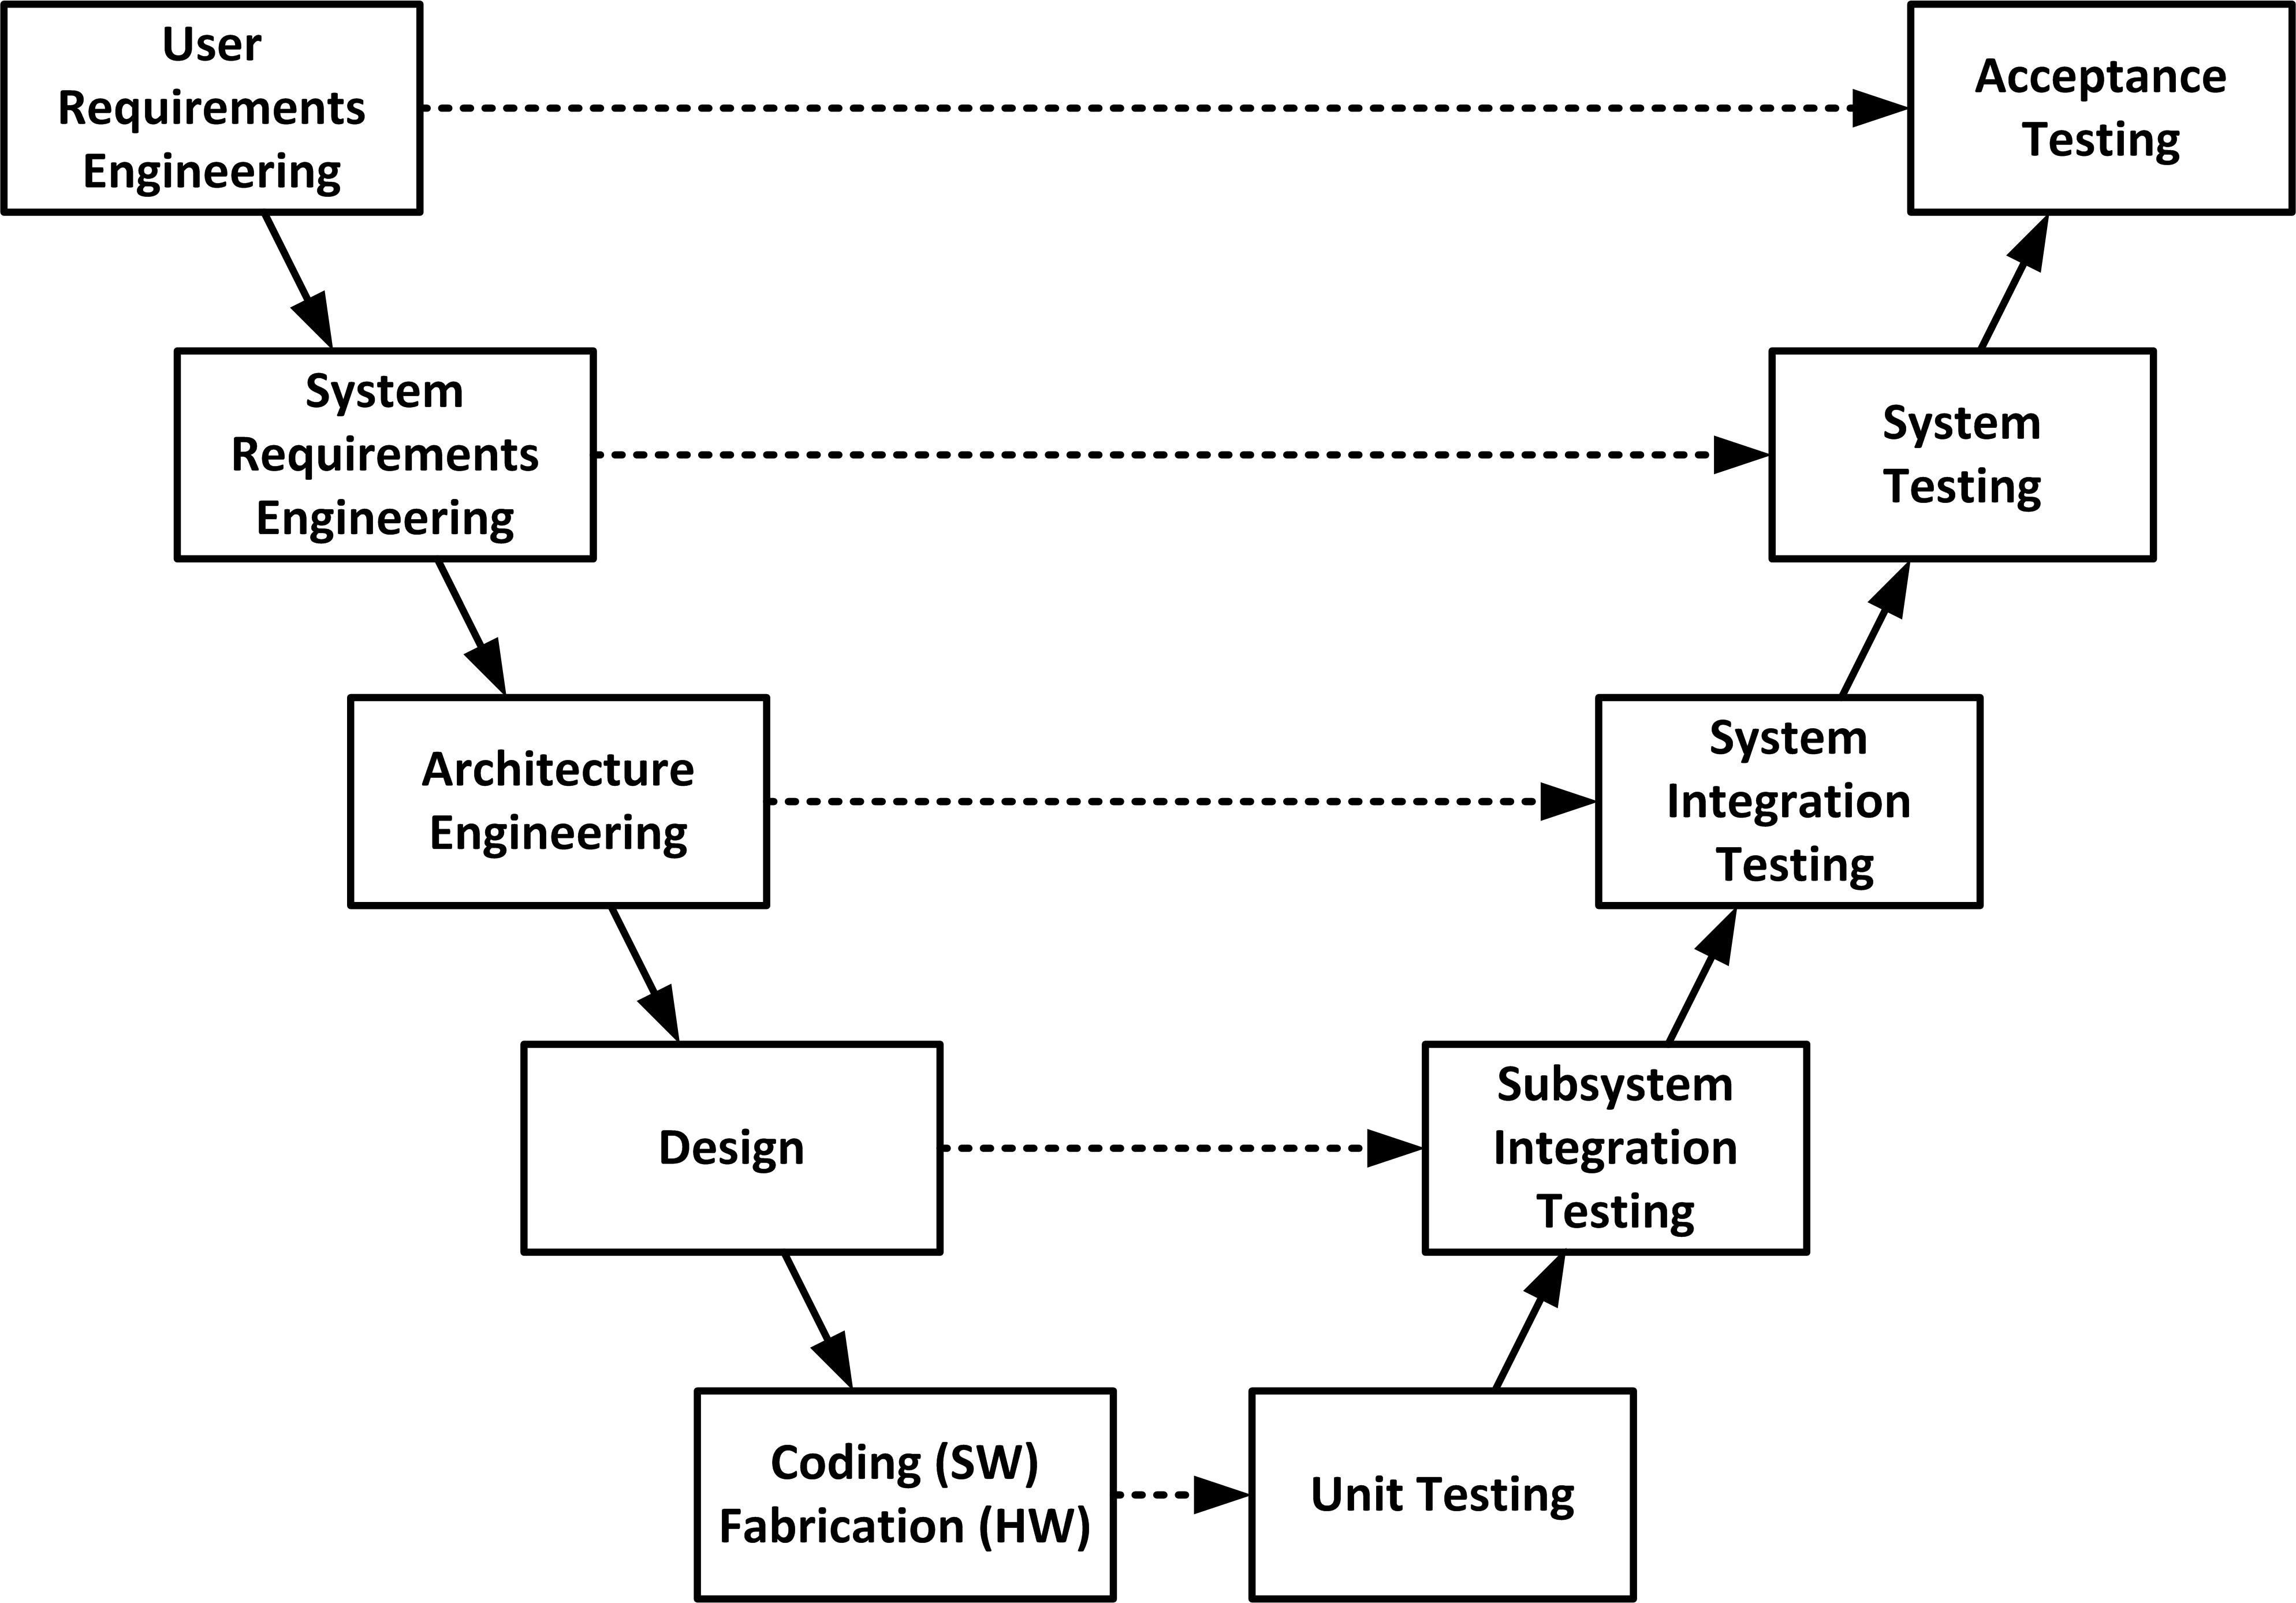
\includegraphics[scale=0.6]{res/images/v_model.jpg}
	\caption{Figura esplicativa del \gls{vmodel}\textsubscript{G}}
\end{figure}

\subsection{Test di accettazione}

\subsection{Test di sistema}

\subsection{Test di integrazione}

\subsection{Test d'unità}

\subsection{Resoconto attività di verifica}
\subsubsection{Esiti dell'indice di Gulpease}
